\begin{frame}{Meta-Evaluation Strategies}
    \begin{definition}[System-level Correlation ($K^{\textrm{sys}}_{m_1,m_2}$)]
        This strategy measures \textbf{how suited $m_1$ is w.r.t.\ $m_2$ if used to compare the performance of two systems}. The correlation is applied to the mean values over all stories for all systems for both measures. Formally:
        \begin{align}
        K^{\textrm{sys}}_{m_1,m_2} & \coloneqq K \left(\frac{1}{N} \mathbf{C}^{\textrm{sys}}_{m_1},\frac{1}{N} \mathbf{C}^{\textrm{sys}}_{m_2} \right),\\
        \text{where} \quad \mathbf{C}^{\textrm{sys}}_{m} & \coloneqq \left[ \sum\limits_{i=1}^N m\left(y_i^1\right),\dots, \sum\limits_{i=1}^N m\left(y_i^S\right)\right].\nonumber
        \end{align}
    \end{definition}
\end{frame}

\begin{frame}{Meta-Evaluation Strategies}
    \begin{definition}[Overall Correlation ($K^{\textrm{ovl}}_{m_1,m_2}$)]
        This strategy measures \textbf{how $m_1$ and $m_2$ agree at the level of the story itself}. It computes the correlation between the full vectors containing the scores of $m_1$ or $m_2$ for a given story for every system. Formally:
        \begin{align}
        K^{\textrm{ovl}}_{m_1,m_2} & \coloneqq K \left( \mathbf{C}^{\textrm{ovl}}_{m_1},\mathbf{C}^{\textrm{ovl}}_{m_2} \right),\\
        \text{where} \quad \mathbf{C}^{\textrm{ovl}}_{m} & \coloneqq \left[\left(m\left(y_i^j\right)\right)_{(i,j) \in \{1, \dots, N\} \times \{1, \dots, S\}}\right].\nonumber
        \end{align}
    \end{definition}
\end{frame}

\begin{frame}{Statistical Testing}
    Correlations between two measures on the same dataset are not independent. We use the Williams test to evaluate the strength of an \textbf{increase} in dependent correlations.
    \begin{definition}[Williams Test]
        Given three features $X_1$, $X_2$ and $X_3$ of a population of size $n$, Williams's $t$ test for whether the correlation between $X_1$ and $X_2$ equals the correlation between $X_1$ and $X_3$ is formulated as follows:
        \[ t \coloneqq \frac{(r_{12} - r_{13}) \sqrt{(n-1)(1+r_{23})}}{\sqrt{2K \frac{(n-1)}{(n-3)} + \frac{(r_{12} + r_{13})^2}{4} (1 - r_{23})^3}} \, , \]
        where $r_{ij}$ is the correlation between $X_i$ and $X_j$ and
        \[ K \coloneqq 1 - {r_{12}}^2 - {r_{13}}^2 - {r_{23}}^2 + 2 \, r_{12} \, r_{13} \, r_{23} \, . \]
    \end{definition}
\end{frame}

\begin{frame}{Statistical Testing}
    Since we perform a large quantity of tests, we need to correct $p$-values for multiplicity. We choose to control the false discovery rate using the Benjamini-Hochberg method.
    \begin{definition}[Benjamini-Hochberg (BH) Method]
        Given $m$ $p$-values $p_1, \dots, p_m$ sorted in increasing order and a significance level $\alpha$, the Benjamini-Hochberg method consists in finding the largest $k$ such that $p_k \leq \frac{k}{m} \alpha$. The null hypothesis would then be rejected for the first $k$ tests. This is equivalent to computing adjusted $p$-values $p_k^\star = p_k \frac{m}{k}$ and replacing the $p$-values from largest to smallest.
    \end{definition}
\end{frame}

\begin{frame}{Statistical Testing}
    \begin{figure}[!h]
        \centering
        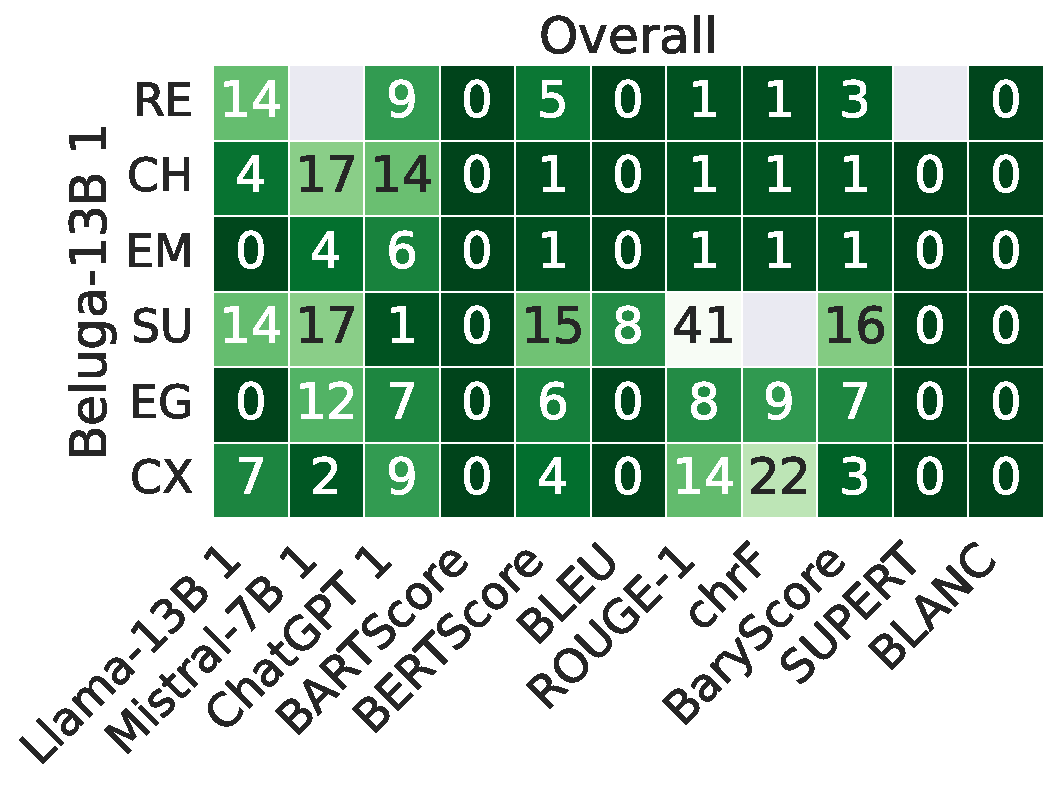
\includegraphics[width=0.6\columnwidth]{pictures/llm_williams_kendall_story_bh.pdf}
        \caption{BH-adjusted $p$-values ($\times$100) of the Williams tests for overall Kendall correlations. Lower is better. ``0'' means $p<0.01$.}
        \label{fig:williams_beluga_story}
    \end{figure}
    \vspace*{-0.4cm}
    Moderate to strong statistical evidence that Beluga-13B correlates better with human judgment than other measures.
\end{frame}

\begin{frame}{Statistical Testing}
    \begin{figure}[!h]
        \centering
        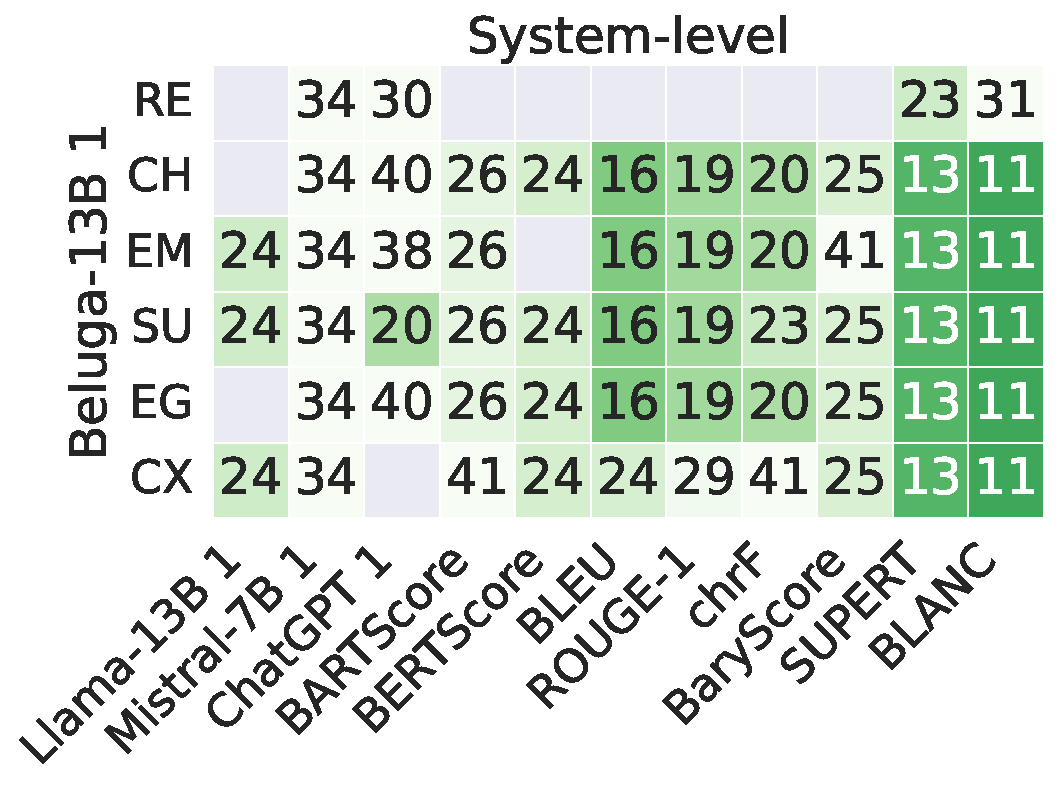
\includegraphics[width=0.6\columnwidth]{pictures/llm_williams_kendall_system_bh.pdf}
        \caption{BH-adjusted $p$-values ($\times$100) of the Williams tests for system-level Kendall correlations. Lower is better. ``0'' means $p<0.01$.}
        \label{fig:williams_beluga_system}
    \end{figure}
    \vspace*{-0.4cm}
    Weaker statistical evidence at the system-level, mitigated by the averaged nature of the correlations.
\end{frame}

\begin{frame}{Influence of Pretraining Data}
    We use the \minkprob\ detection method \citep{shi2023detecting} which is based on the hypothesis that unseen data will contain more outlier words with low probability than seen data. Given a sequence of tokens $x = x_1, \dots, x_N$ and an LLM's probability distribution $p$ of the next token, \minkprob\ selects the top-$k$\% of tokens with the highest negative log-likelihood to form a set \mink(x) and computes their average log-likelihood. Formally:

    \[ \minkprob (x) \coloneqq \frac{1}{E} \sum_{x_i \in \textrm{Min-K\%}(x)} \log p \left(x_i \mid x_1, \dots, x_{i-1} \right) ,\]
    
    where $E$ is the size of the \mink(x) set. We can then detect if the sentence was included in pretraining data by thresholding this average. We follow \citet{shi2023detecting} and use $k=20$ for our two experiments.
\end{frame}

\begin{frame}{Influence of Pretraining Data}
    We use the {\minkprob} detection method to verify whether the LLMs were trained on the {\wpfan} dataset.
    \begin{table}[h]
        \centering
        \begin{tabular}{lr}
        \toprule
        \textbf{Model} & \textbf{Contamination (\%)} \\
        \midrule
        Platypus2-70B & 0.80 \\
        Llama-30B & 1.80 \\
        Beluga-13B & 4.40\\
        Mistral-7B & 2.50 \\
        Llama-7B & 10.10\\
        \bottomrule
        \end{tabular}
        \caption{Predicted contamination rates of a random {\wpfan} sample of 1,000 stories.}
        \label{tab:wp_contamination}
    \end{table}
    \vspace*{-0.4cm}
    The low predicted rates suggest this was not the case.
\end{frame}

\begin{frame}{Influence of Pretraining Data}
    We use the {\booksmia} dataset to compute the area under the ROC curve (AUC) obtained with \minkprob\ thresholding.
    \begin{table}[h]
        \scriptsize
        \centering
        \begin{tabular}{lc}
        \toprule
        \textbf{Model} & \textbf{AUC (\%)} \\
        \midrule
        Platypus2-70B & 92.1 \\
        Llama-30B & 81.3 \\
        Beluga-13B & 70.1\\
        Mistral-7B & 51.2 \\
        Llama-7B & 55.1 \\
        \bottomrule
        \end{tabular}
        \caption{AUC detection score on the {\booksmia} dataset}
        \label{tab:book_auc}
    \end{table}
    \vspace*{-0.3cm}
    The higher AUC detection score for larger models means that \textbf{it is easier to detect if a book was in the training data of a larger LLM}, and that larger LLMs tend to produce text that is \textbf{more faithful to their training data}. This could explain their better ASG performance.
\end{frame}

\begin{frame}{Environmental Impact}
    \begin{itemize}
        \item We used the Jean Zay supercomputer;
        \item A100 GPU nodes: 1,431 hours consumed;
        \item V100 GPU nodes: 203 hours consumed;
        \item Estimation balance sheet: 0.078 tons of CO2 equivalent, according to the Labos 1point5 estimation method\footnote{\scriptsize \url{https://labos1point5.org/les-rapports/estimation-empreinte-calcul}};
        \item $\approx$ a one-way Paris-Marseilles flight.
    \end{itemize}
\end{frame}

\begin{frame}{On LLM Intelligence: Playing Chess}
    Interesting work from \citet{karvonen2024emergent}: ``we provide evidence that an \textbf{LLM trained on a next token prediction task can develop a world model of complex systems such as chess}, including the ability to estimate latent variables such as player skill.'' Their best linear probe classifier achieves \textbf{99.6\% accuracy} in classifying the precise state of each square across 10,000 test games.
    \begin{figure}
        \centering
        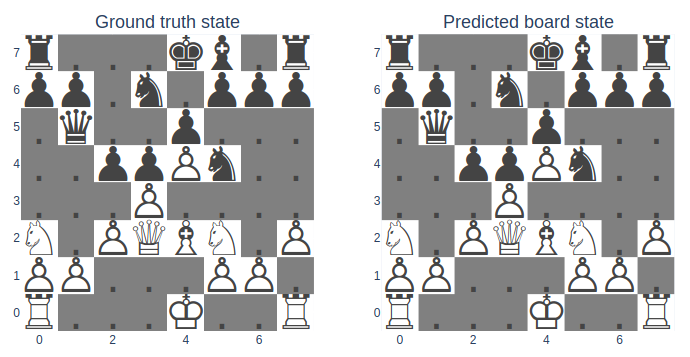
\includegraphics[width=0.8\linewidth]{pictures/board_state.png}
        \label{fig:chess_board_states}
    \end{figure}
\end{frame}

\begin{frame}{Quality Criteria for Evaluations Taxonomy}
    \citet{belz-etal-2024-qcet-interactive} attempt to standardize quality criteria in NLP with an interactive tool:
    \begin{enumerate}
        \item First node of the taxonomy: Overall Quality;\
        \item Correctness / Goodness / Features;
        \item In Their Own Right / Relative to the Inputs / Relative to an External Frame of Reference;
        \item Form / Content / Form and Content;
    \end{enumerate}
    But the tool was unavailable online...?
\end{frame}

\begin{frame}{Manual Annotation}
    \citet{lee-etal-2019-best} advise to:
    \begin{itemize}
        \item use quantitative analysis ``if the goal is to judge the merit of the system'';
        \item use ``either multiple-item 7-point Likert scales, or a (continuous) ranking task'';
        \item ``choose a sample that reflects the audience for which the system was developed''.
    \end{itemize}
    \citet{karpinska2021perils} show that ``AMT worker judgments improve when they are shown model-generated output alongside human-generated references, which enables the workers to better calibrate their ratings''.
\end{frame}

\begin{frame}{Initial PhD Topic (April 2021)}
    Recent advances in natural language processing have enabled language models to produce ever more realistic texts. However, automatically generated texts exhibit poor consistency; we argue that this is due to the lack of a strong representation of the underlying state of the story. This thesis will study the \textbf{extraction and representation of a meaningful chain of events} from a given text, and, reciprocally, the \textbf{generation of a convincing story from such a representation}. We will also study the \textbf{controllability of the generated text}; for instance by enforcing formal constraints such as the respect of poetic conventions.
\end{frame}